\documentclass{article}%
\usepackage[T1]{fontenc}%
\usepackage[utf8]{inputenc}%
\usepackage{lmodern}%
\usepackage{textcomp}%
\usepackage{lastpage}%
\usepackage[head=40pt,margin=0.5in,bottom=0.6in]{geometry}%
\usepackage{graphicx}%
%
\title{\textbf{Tasa de mortalidad infantil en Venezuela incrementó durante el año 2017}}%
\author{El Nacional Web}%
\date{02/10/2018}%
%
\begin{document}%
\normalsize%
\maketitle%
\textbf{URL: }%
http://www.el{-}nacional.com/noticias/crisis{-}humanitaria/tasa{-}mortalidad{-}infantil{-}venezuela{-}incremento{-}durante{-}ano{-}2017\_254097\newline%
%
\textbf{Periodico: }%
EN, %
ID: %
254097, %
Seccion: %
Crisis humanitaria\newline%
%
\textbf{Palabras Claves: }%
Crisis humanitaria, Sociedad\newline%
%
\textbf{Derecho: }%
2.1%
, Otros Derechos: %
NO\_TIENE%
, Sub Derechos: %
2.1.1%
\newline%
%
\textbf{EP: }%
NO\newline%
\newline%
%
\textbf{\textit{Unicef ha expresado en varias ocasiones su preocupación ante el incremento de este flagelo}}%
\newline%
\newline%
%
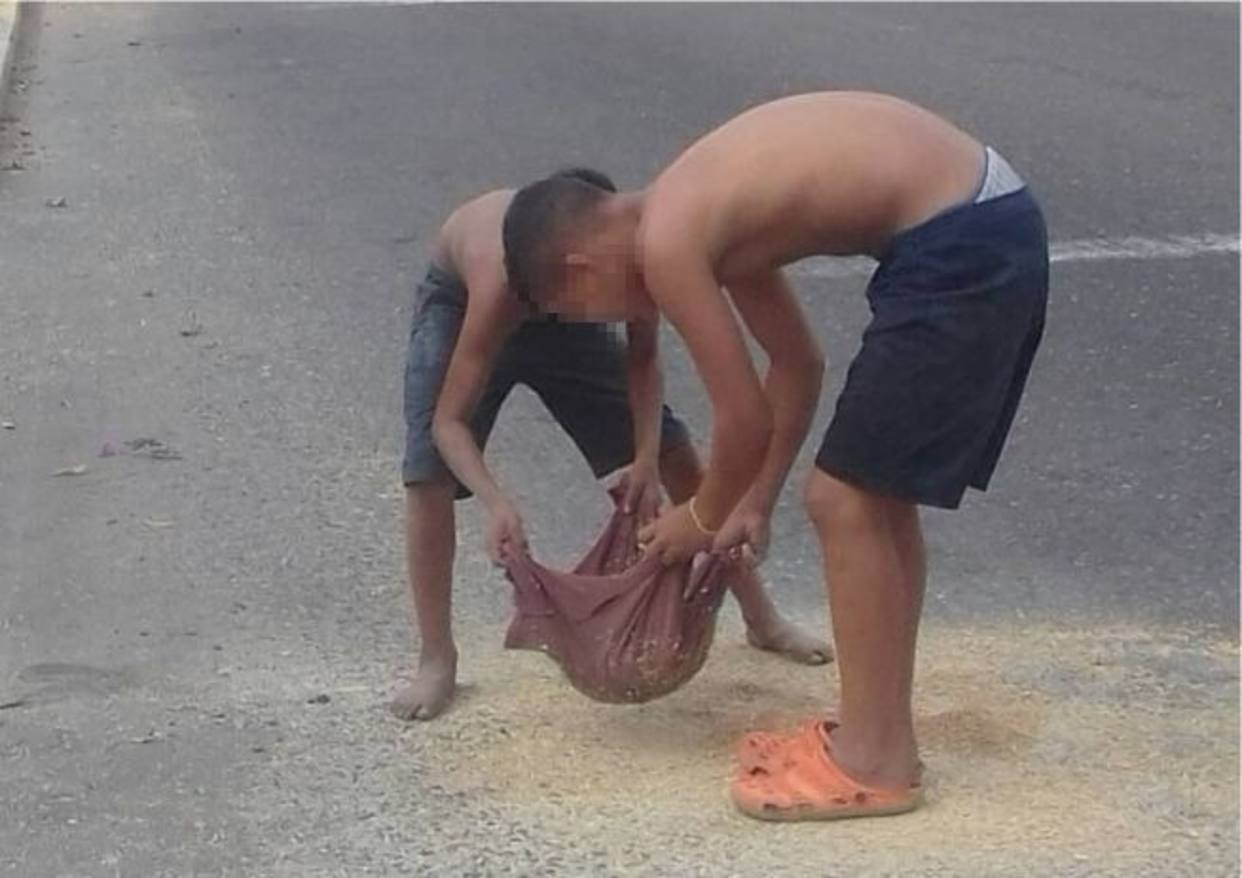
\includegraphics[width=300px]{30.jpg}%
\newline%
%
Un estudio realizado por El Fondo de las Naciones Unidas para la infancia (Unicef) y que fue publicado en septiembre indicó que la mortalidad infantil de menores de cinco años se incrementó en Venezuela durante el año 2017 con respecto a los niveles registrados en 1990.%
\newline%
%
La investigación del organismo multilateral señaló que, en 1990, la tasa de mortalidad de niños se ubicó en 60 muertes por cada 1.000 recién nacidos, mientras que en 2017 la cifra aumentó a 61 muertes por cada 1.000 nacimientos.%
\newline%
%
En 1990 se registraron 14 mil muertes de niños, en comparación con las 15 mil muertes registradas en 2017.%
\newline%
%
En el informe de Unicef se observó también que la tasa de mortalidad neonatal aumentó de 7 mil muertes por cada 1.000 recién nacidos en 1990 a 12 mil muertes por cada 1.000 en 2017.%
\newline%
%
El organismo adscrito a la Organización de las Naciones Unidas ha expresado en varias ocasiones su preocupación ante el incremento de la mortalidad infantil en Venezuela, y ha reiterado su disposición para~apoyar al país para frenar lo que ha calificado como una crisis sanitaria en el país.%
\newline%
%
Con información de~Unicef%
\newline%
%
\end{document}